\documentclass[a4paper,11pt]{article}
\usepackage[margin=2cm]{geometry}
\usepackage{graphicx}

\usepackage{xeCJK}
\setCJKmainfont[ItalicFont={SimHei}]{SimHei}
\setCJKsansfont{SimHei}
\setCJKmonofont{SimHei}

\renewcommand{\figurename}{图}

\title{匹兹堡附近2015-04至2016-03气象数据和简要分析}
\author{HMW-Alexander}

\begin{document}

\maketitle

\begin{figure}[!htb]
\centering
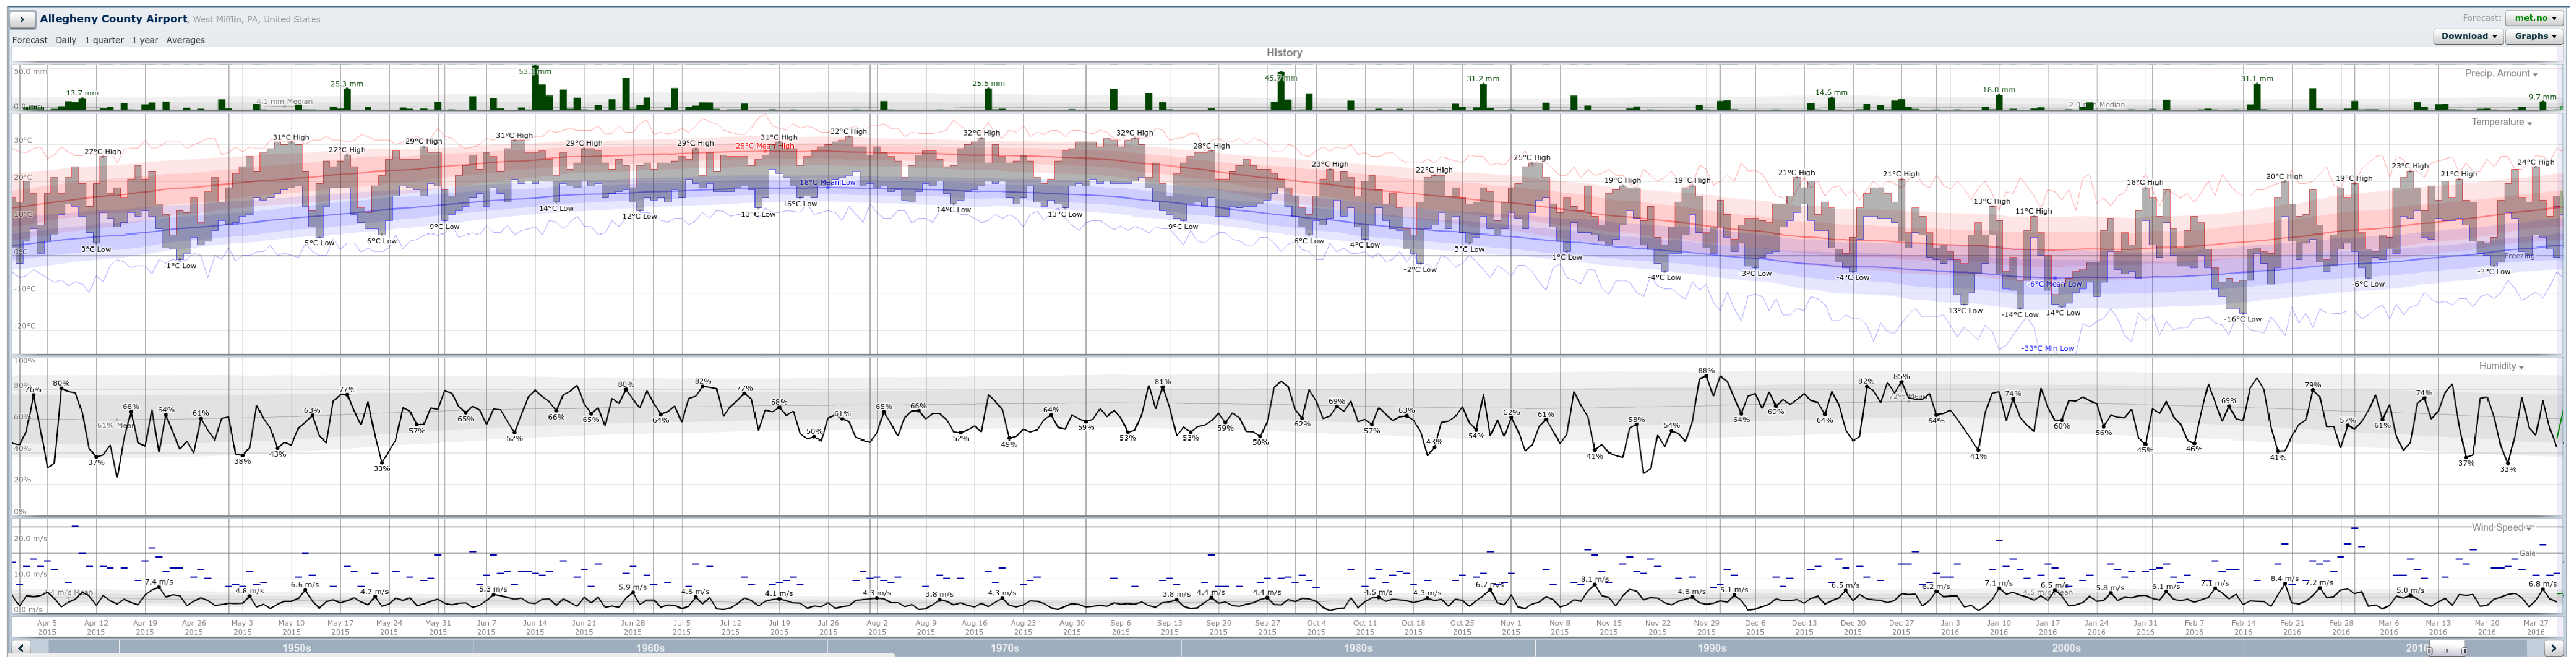
\includegraphics[width=0.9\textwidth]{data}
\caption{阿利根尼县机场气象站数据图(2015-04至2016-03).第一行:降水量;第二行:气温;第三行:湿度;第四行:风速。图片为高清图片,可以放大查看细节。(本数据图没有获得发布权限,仅限内部交流,请勿转载)}
\end{figure}

\begin{figure}[!htb]
\centering
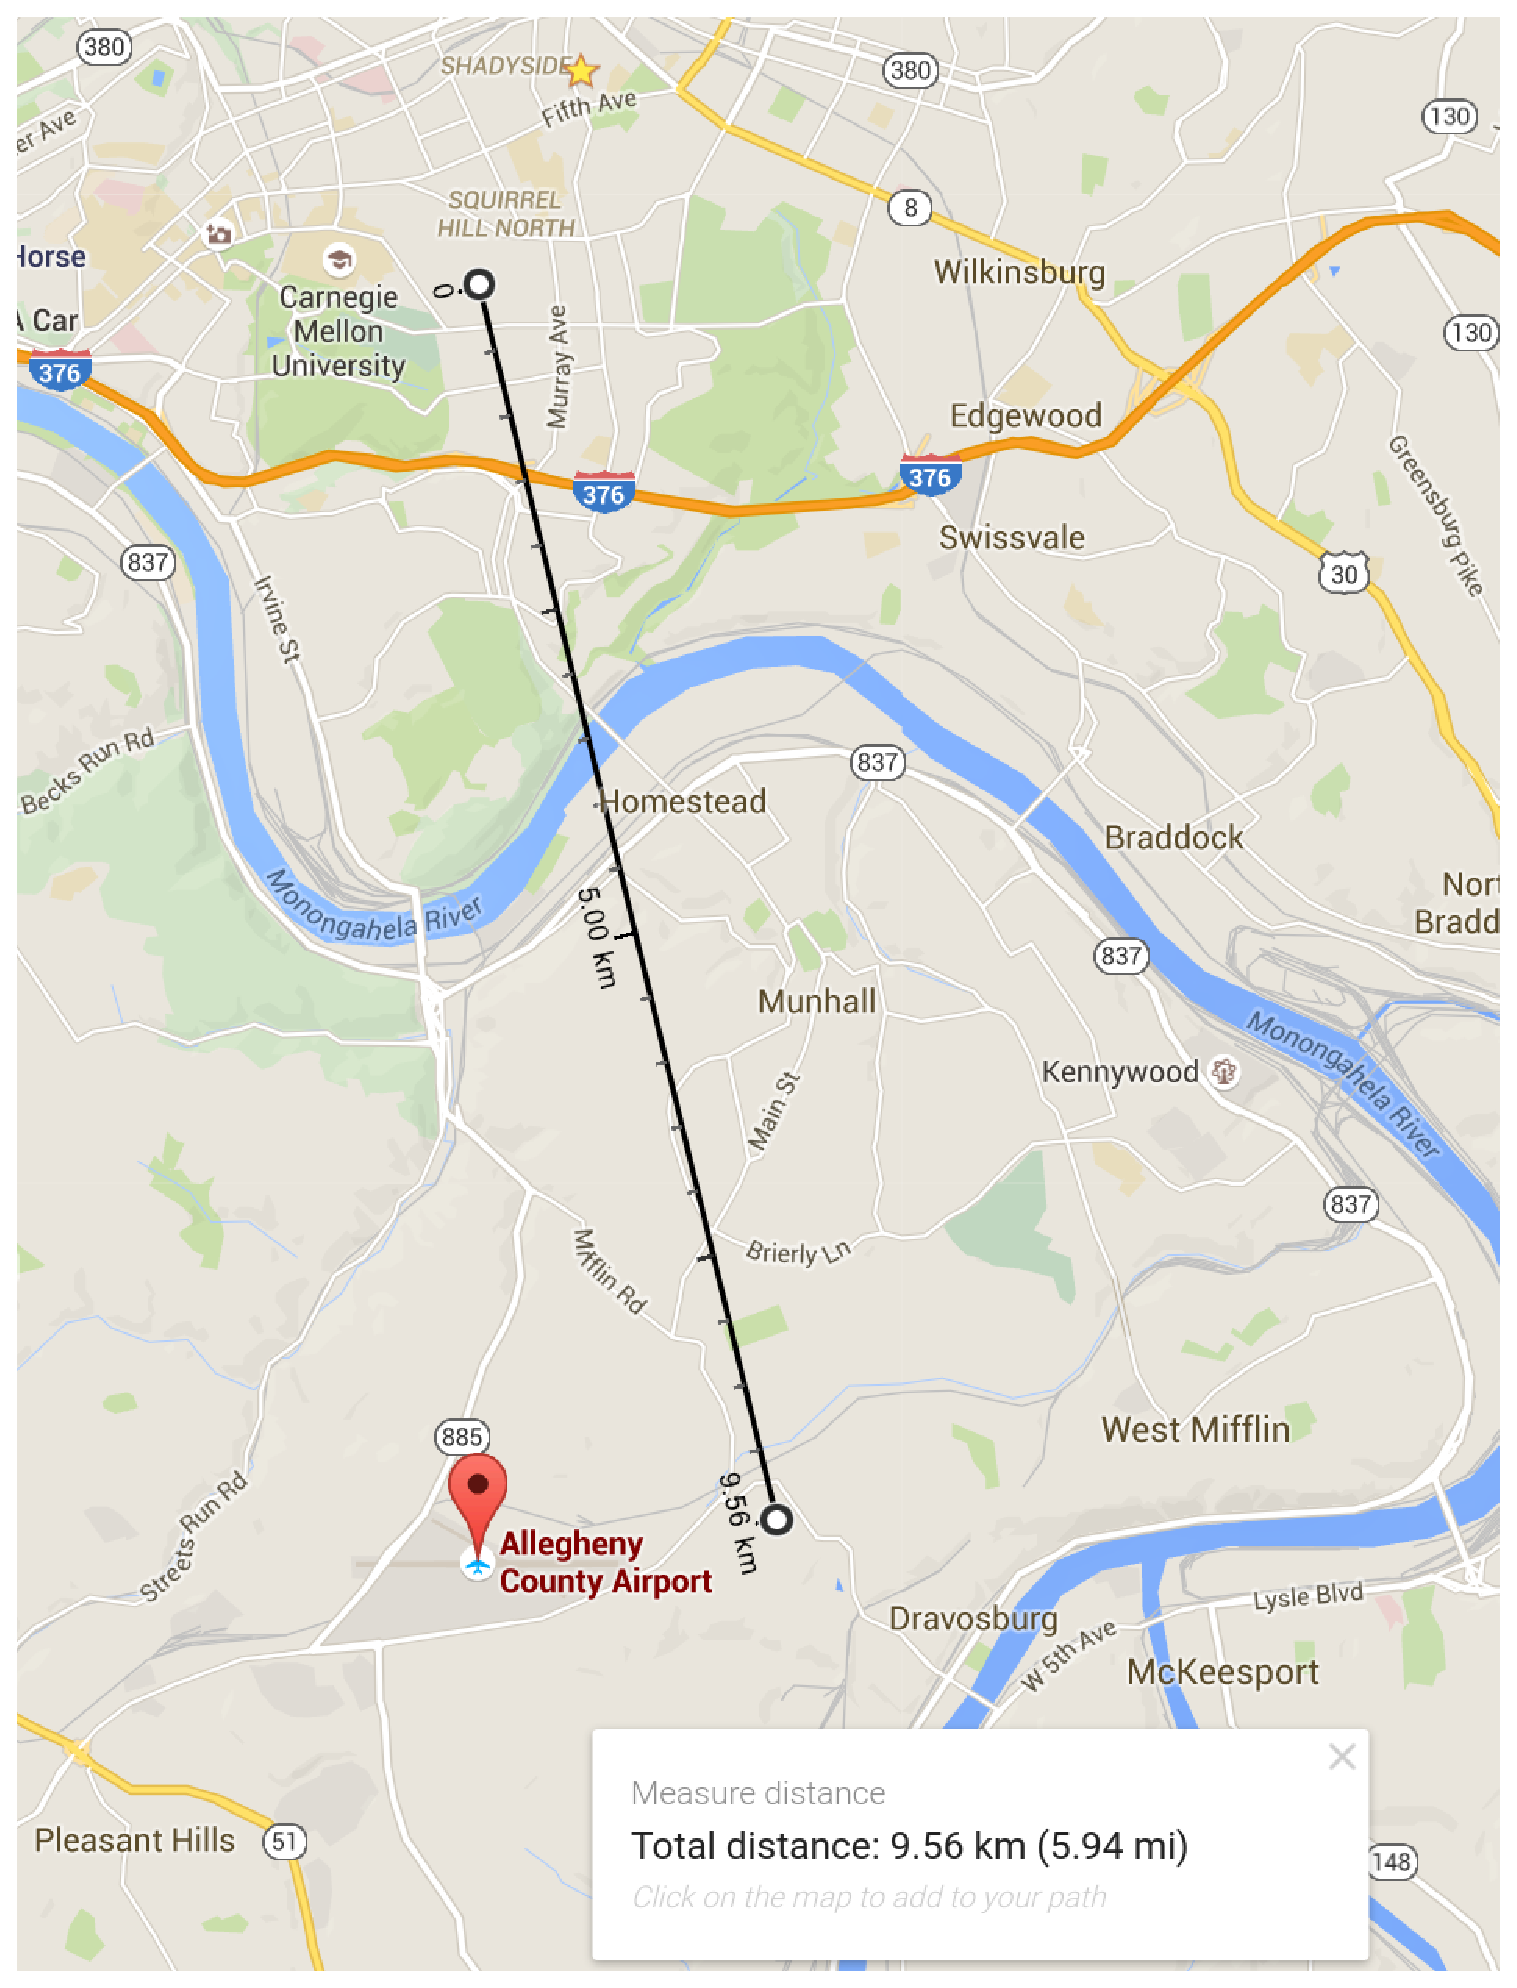
\includegraphics[width=0.3\textwidth]{loc}
\caption{阿利根尼县机场位于CMU南10公里。(© 2016 Google Inc, used with permission. Google and the Google logo are registered trademarks of Google Inc.)}
\end{figure}

个人分析\footnote{为个人从数据上的分析,可能与实际情况不符,仅供参考。}:
\begin{itemize}
	\item 去年最低气温为零下16摄氏度,所以确实是非常冷的。
	\item 由秋转冬,天气变冷的时候,湿度很不幸地呈上升趋势(主要因为趋于频繁的降水/雪),大概分布在50\%到80\%,所以单从数据上来看,匹兹堡的冬天是较为潮湿的。
	\item 风速主要分布在3到4级(3-8 m/s)有时能到5级,所以风速通常来说不大。
	\item 因此建议大家找房的时候尽量避免住在较低楼层,因为阴冷潮湿的冬天会使房内湿气较重,长时间对身体非常不好\footnote{本人在日本东海岸城市的亲身经历,一个湿冷的冬天(零下5摄氏度左右,湿度80\%左右)就扛不住了(当然有点作死的睡在榻榻米上)。}。当然现在的空调大多有除湿功能,需要的时候不要忘记使用。
\end{itemize}

\end{document}